\documentclass[en,hazy,blue,screen,14pt]{elegantnote}
\usepackage[T1]{fontenc}
\usepackage[latin9]{inputenc}
\usepackage{babel}
\usepackage{float}
\usepackage{textcomp}
\usepackage{amsmath,amsfonts,amssymb}
\usepackage{amsthm}
\usepackage{graphicx}
%\usepackage[ruled,vlined]{algorithm2e}
\PassOptionsToPackage{normalem}{ulem}
\usepackage{ulem}
\usepackage{cancel}
\usepackage{mathtools}
\usepackage{url}
\usepackage{hyperref}
\usepackage{algorithm, algpseudocode}

\renewcommand\qedsymbol{$\blacksquare$}
\DeclarePairedDelimiter{\ceil}{\lceil}{\rceil}
\newcommand\tab[1][1cm]{\hspace*{#1}}
\newenvironment{claim}[1]{\par\noindent\underline{Claim:}\space#1}{}
\newenvironment{claimproof}[1]{\par\noindent\underline{Proof:}\space#1}{\hfill $\blacksquare$}
\renewcommand{\algorithmicrequire}{\textbf{Input:}}
\renewcommand{\algorithmicensure}{\textbf{Output:}}

\title{Class Notes\\CIS 502 Analysis of Algorithm\\8-Approximation and Optimization}
\author{Da Kuang}
\institute{University of Pennsylvania}
% \version{1.00}
\date{}

\begin{document}

\maketitle
\newpage
% \input{}
\section{Vertex Cover Approximation}
Given a graph $G=(V,E)$, a vertex cover is a subset $S \subseteq V$, so that for each edge $(u,v) \in E$ at least one of $u$ or $v$ lies in $S$.

Vertex cover decision problem (VC):
\begin{itemize} 
	\item Instance: graph $G$, integer $k$
	\item Question: does $G$ have a vertex cover of size at most $k$?
\end{itemize}

\subsection{Approximation Algorithm}
VC-OPT:
\begin{itemize}
	\item Instance: Graph $G$
	\item Goal: Find the size of the smallest vertex cover in $G$.
\end{itemize}

Exercise: Show how to finding the size of the vertex cover allows you to find the VC of that size.

Instance $I$ is just a graph. OPT($I$) = size of the subset VC in $I$. Let $A$ be any algorithm that find some vertex cover in a given instance $I$. Let $A(I)$ be the size of the vertex cover returned by $I$. If $A$ solve VC exactly then $A(I)$ = OPT($I$) $\forall I$. $A$ is a c-approximation algorithm if $\frac{A(I)}{OPT(I)} \le C, \forall I$. If $A$ is an exact optimization algorithm, then $c = 1$. Efficient algorithm $A$ may not achieve $c = 1$. We want $A$ that achieves a small approximation factor $\ge 1$.

Suppose we can lower bound the value of OPT($I$) for each $I$. Let $\ell (I) \le OPT(I) \forall I$. If we can prove that $\frac{A(I)}{\ell(I)} \le c$ for some $c$, then $\frac{A(I)}{OPT(I)} \le c$.

Given the following graph $I$, how to find the lower bound of OPT($I$).
\begin{figure}[H]
	\centering
	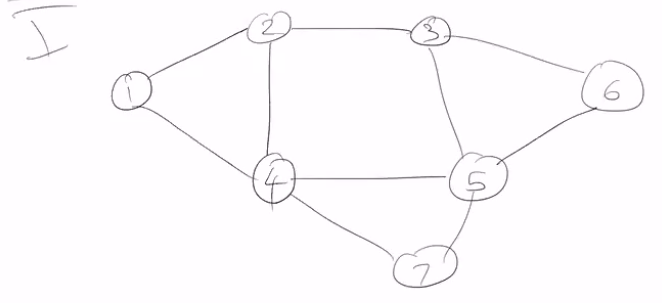
\includegraphics[width=0.5\textwidth]{fig/vc-low-bound.png}
\end{figure}

Matching is a set of edges that do not share any end point. The size of a matching is a lower bound on the size of a vertex cover. If on an instance $I$, we find a matching $M$, then the size VC $\ge |M|$. 

Note that maximal and maximum are two different concepts:
\begin{itemize}
	\item Maximal matching in a graph $I$ is a matching $M$ that cannot be extended. i.e, cannot add any edge to $M$ and still have a matching.
	\item Maximum matching is the matching set with the biggest set.
\end{itemize}

For example, in the following graph, red edges consist of a maximum matching while the green edge is a maximal matching by itself. It is because we are not able to expand any more after choosing the green edge. If we choose randomly, most of time we may end up with maximal matching instead of maximum. But maximal matching is actually enough for lower bound approximation.
\begin{figure}[H]
	\centering
	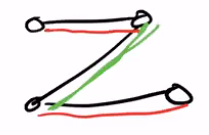
\includegraphics[width=0.3\textwidth]{fig/vc-max.png}
\end{figure}
Size of maximal matching is a lower bound on the size of the vertex cover. In the following example, black edges form a maximal matching.
\begin{figure}[H]
	\centering
	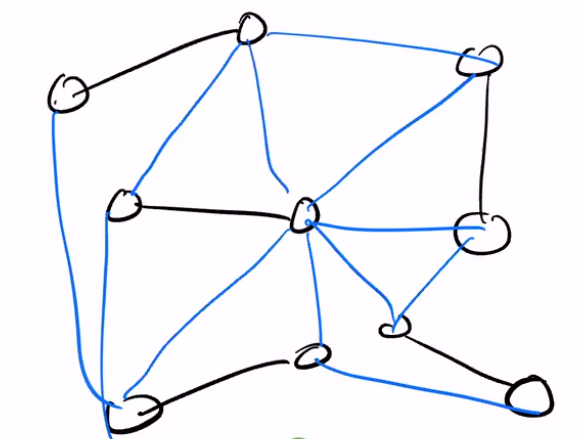
\includegraphics[width=0.3\textwidth]{fig/vc-matching.png}
\end{figure}

If $(u, v)$ is an edge that is not in the maximal matching, either $u$ or $v$ musts be an end point of some matching edge. In the opposite case, could you have an edge $(u, v)$, neither of whose end points has been matched into the maximal matching. The answer is no, since if such edge exist, we could actually add it into the maximal matching.

Find the vertex cover as follows: find a maximal matching $M = \{(u_1, v_1), (u_2, v_2) \cdots , (u_k, v_k)\}$. Pick all $2k$ vertices that are end points of edges in $M$. This is a vertex cover.

\subsection{Proof}
Suppose for contradiction, $\exists (u, v):$ neither $u$ nor $v$ $\in$ matching $M = \{u_1, u_2, \cdots, u_k, v_1, \cdots, v_k\}$. Then $(u, v)$ could have been added to $M$, contradicting the fact that $M$ is maximal.

Lower bound on the size of a vertex cover is $k$.

Our algorithm produces a C-approximation for $c = \frac{2k}{k} = 2$. 

Given graph $I$: how to find a maximal matching?  

A greedy algorithm works. Arrange edges in arbitrary order $e_1, e_2, \cdots, e_m$. $M = \emptyset$. For $i = 1$ to $m$, if $M \cup {e_i}$ is a matching, then $M = M \cup {e_i}$.

Could there be an edge $(u, v)$ in $I$ such that $M$ could be extended by $(u, v)$? The answer is NO. So $M$ is a maximal matching.

In conclusion, 2-approximation for VC given instance $I$:
\begin{itemize}
	\item find the maximal matching $M$
	\item output the set of of vertices consisting of both end points of each edge in $M$.
\end{itemize}
























































\section{Metric Traveling Salesman Approximation}
Given $n$ cities that the traveling sellsman want to do business, matrix $M$ where $M_{ij}$ is the distance from city $i$ to city $j$. The goal is to find a tour of $n$ cities returning to the starting cities of least total cost.

Describe the problem mathematically, find a permutation $\sigma$ of $1 \cdots n$ so as to minimize \[\sum_{i=0}^{n-1} M[\sigma(i), \sigma(i+1)] + M[\sigma(n), \sigma(1)]\]

This is a NP-hard problem. 

The decision problem is NP complete:
\begin{itemize}
	\item Instance: matrix $M$ and a budge $B$
	\item Question: is there a tour of the cities with cost at most $B$.
\end{itemize}

The problem is in NP. Given a permutation of cities as certificate, we can check the cost in order and sum the cost up to see if it is lower than the given budge. It can be finished within polynomial time.

Prove NP-complete by a reduction from Hamilton cycle (HAMCYCLE).

The Hamilton cycle decision problem(HAMCYCLE):
\begin{itemize}
	\item Instance: directed graph $G$
	\item Question: is there a simple cycle containing all the vertices? (such cycle is called a Hamilton cycle)
\end{itemize}

Exercise: HAMCYCLE $\preccurlyeq_P$ TSP.

\subsection{Approximation Algorithm TSP OPT}
Don't know a good approximation for a general TSP.  But we are able to approximate Metric -TSP. Metric TSP is as follow:
\begin{itemize}
	\item Input: matrix $M$ of costs. $M$ satisfies the property of a metric:
	\begin{itemize}
		\item $M[i, i] = 0$
		\item $M[i, j] = M[j, i]$
		\item $M[i, k] \le M[i, j] + M[j, k], \forall i, j, k$.
	\end{itemize} 
\end{itemize}
 
OPT(M) is the cost of the best tour for a given matrix $M$. Design algorithm $A$. We say $A(M)$ is the cost of tour that $A$ outputs. We want $\forall M, \frac{A(M)}{OPT(M)} \le C$. Can achieve $c = 2$.

Suppose we have a best tour, when we delete one edge from the tour, what do we have? We get a Hamilton path which goes through all the cities. The path is a tree on all the vertices in the graph, i.e. a spanning tree. The cost this spanning tree (path) $\le$ cost of the tour. So cost of MST $\le$ cost of the spanning tree $\le$ cost of the optimal tour.

Approximation algorithm:
Think of $M$ as a weighted, connected,  undirected graph. Find the MST in the graph, call it $T$. Duplicate every edge in $T$. Cost of $T$ $\le$ cost of OPT. The cost of duplicated tree = 2 $\times$ cost$(T)$.

Because of the duplication, every vertex has even degree. So any connected undirected graph with all degrees even has an Eulerian tour. Eulerian tour is a tour that goes though all the edges of the graph exactly once. We can find Eulerian efficiently in order $O(m+n)$ time using DFS.

\begin{figure}[H]
	\centering
	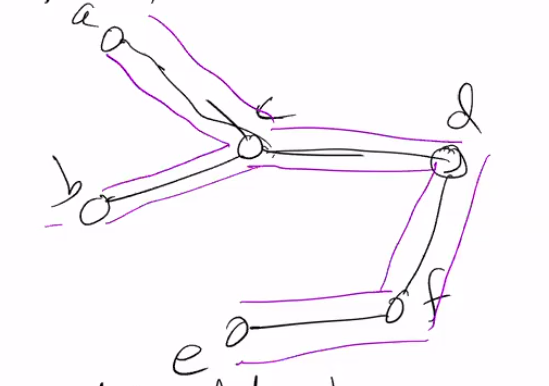
\includegraphics[width=0.5\textwidth]{fig/eulerian-tour.png}
\end{figure}

The Eulerian tour in the above graph is $(a, c, d, f, e, f, d, c, b, c, a)$. 

The cost of Eulerian tour = $2 \times$ MST $\le$ 2 OPT($M$). So it turns out the Eulerian tour is a nice tour with the cost less than 2 OPT($M$). But we cannot use Eulerian as the output since the real undirected graph does not have duplicate edges. But it is easy to generate Hamilton path from Eulerian tour by skip the duplicates. To be more specific, drop the edges in Eulerian tour as long as it has been seen before.

Therefore the Hamilton tour is $(a, c, d, f, e, \cancel{f, d, c,} ~b~\cancel{, c, a})$

\textbf{Claim}: Removing duplicate occurrences of vertices in the Eulerian tour dose not increase the cost of the tour.

\begin{proof}
	\begin{figure}[H]
		\centering
		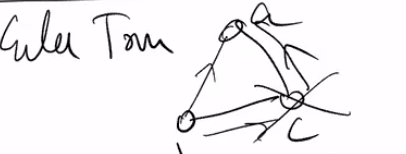
\includegraphics[width=0.3\textwidth]{fig/trangle.png}
	\end{figure}
If we remove $c$ from the graph and connect b to a, recall that this is a metric matrix so the triangle rules applies. $M[b, a] \le M[b, c] + M[c, a]$.

We then use induction to prove that $(e,b)$ is less than $(b, c, d, f, e)$.
\begin{figure}[H]
	\centering
	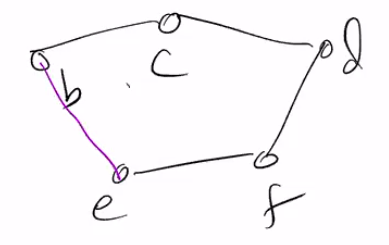
\includegraphics[width=0.3\textwidth]{fig/trangle-short-path.png}
\end{figure}

First of all, if we only skip vertex $f$ by connecting $e$ to $d$. $(e, d)$ would be better than $(e, f, d)$ by triangle rules. Then use the same idea again . $(e, c)$ would be at most expensive as $(e, d, c)$. Then finally $(e,b)$ is better than $(e, c, b)$. This applies more generally for a sequence of vertex deletion.
\end{proof}
\subsubsection{Appro Algorithm}
\begin{itemize}
	\item Find MST ($\le$ OPT)
	\item Duplicate edges ($\le$ 2 OPT)
	\item Find Eulerian tour ($\le$ 2 OPT)
	\item Convert to Hamilton tour (or TSP tour) by skipping duplicate visits to vertices. ($\le$ 2 OPT)
\end{itemize}
This is a 2-approximation algorithm.



\subsection{Improvments}
\subsubsection{Christofides}
Metric-TSP can be approximate even better than 2-approximation. The best known approximation is \textbf{1.5-approximation} for metric-TSP by Christofides Algorithm. 
\begin{itemize}
	\item Find MST ($\le$ OPT)
	\item Christofides: find the min-cost perfect matching on the odd degree vertices. Add it to the MST. Now all the vertices become even degree. ($\le$ 1.5 OPT)
	\item Find Eulerian tour ($\le$ 2 OPT)
	\item Convert to Hamilton tour (or TSP tour) by skipping duplicate visits to vertices. ($\le$ 2 OPT)
\end{itemize}

\begin{figure}[H]
	\centering
	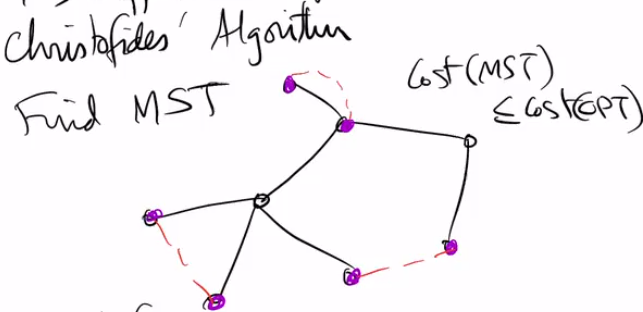
\includegraphics[width=0.5\textwidth]{fig/christofides.png}
\end{figure}
\subsubsection{Approximation Scheme}
Approximation Scheme: given any $\epsilon$ as input, there is an algorithm that always find a solution that is at most $(1 + \epsilon)$ time OPT. Running time of the algorithm grows as a polynomial function of $\frac{1}{\epsilon}$.





















\section{Set Cover Approximation}
\subsection{Set Cover Problem}
Input: Universe of elements $U = \{1, \cdots, n\}$. A collection of subsets of $U$, $\mathfrak{S} = \{S_1, S_2, \cdots, S_m\}$, where each $S_i \subset U$. 

Set cover decision problem: 
\begin{itemize}
	\item Instance: $U$, $\mathfrak{S}$ and given a number $k$.
	\item Question: is there a sub-collection $\mathfrak{f}' = \{S_{i1}, S_{i2}, \cdots, S_{ik}\}$ (at most $k$ sets), such that $\cup_{j=1}^k S_{ij} = U$.
\end{itemize}

Set Cover is in a NP problem. The certificate for a YES-instance is just the sub-collection $\mathfrak{f}'$. It is easy to check whether the sub-collection covers all the elements in the universe and has at most $k$ sets.

Set cover is actually a NP hard problem since it is a generalization of vertex cover problem.


We can show VC reduces to SC in polynomial time. VC $\preccurlyeq_P$ SC. In general, reduce a particular case to a general case would be easy, which is the case in our problem.

Given instance $\langle G, k \rangle$ of VC, we create an instance of set cover as follows:
Let the universe be the set of edges in $G$. $U = \{e_1, e_2, \cdots, e_n\}$. For each vertex $v \in G$, create a subset $S_V = \{e \in E: e \text{ has $v$ as one of its end points.}\}$. Use the same $k$ as the number of vertex sets as the number of sets in SC.
\begin{figure}[H]
	\centering
	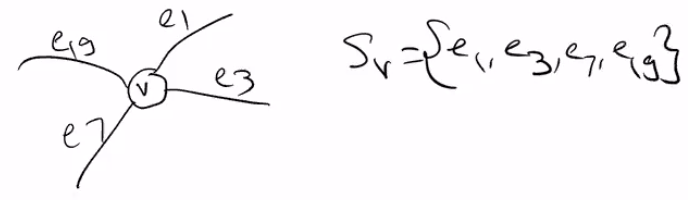
\includegraphics[width=0.5\textwidth]{fig/vs-reduce-to-sc.png}
\end{figure}

If the starting instance is a YES instance of VC, then the reduction produce YES-instance of SC. Conversely, if the instance of SC we produce is a YES instance, then the starting instance must be a YES instance of vertex cover.

\subsection{Set Cover Optimization}

\subsubsection{Greedy Algorithm}
Set Cover Optimization is NP-hard. Approximation algorithm for set cover using a greedy strategy. Recall that the goal is to cover all the vertices. So naturally the first choice of greedy algorithm would be the set that cover as much vertices as possible.

Algorithm $G$:
$R$ is the set of uncovered elements. $C$ is a collection of subset chosen by $G$. Initially, $R = U$ and $C = \emptyset$.

while($R \neq \emptyset$):
\begin{itemize}
	\item pick $S_i$ such that $|S_i \cap R|$ is maximum
	\item $C = C \cup {S_i}$
	\item $R = R - S_i$
\end{itemize}

\subsubsection{Matching Upper Bound of Approximation Factor}
This algorithm can produce a solution that is a factor of $\log n$ which worse than the best possible.

Call our given instance $I = \langle U, C \rangle$. Let OPT($I$) = $k$, be the best number of set that OPT picks on $I$. Say $k = 5$. So OPT covered the whole universe in 5 sets. (see red sets in the following fig). So OPT also covers $R$ in at most 5 sets. (see green sets in the following fig). These is a set in OPT that covers at least $\frac{|R|}{k}$ elements in $R$.

$G$ picks the set that covers the most elements in $R$. So $G$ must pick a set that cover at least $\frac{|R|}{k}$ elements.

After $G$ picks one set, the size of $R$ drops from $|R|$ to at most $|R|(1 - \frac{1}{k})$.

Initially, $|R| = n$. After $G$ has picked $t$ sets. $|R| \le n (1 - \frac{1}{k})^t$. If we get the size of $R$ down to 1, the greedy is essentially finished.

Let's find $t$ such that $n ( 1 - \frac{1}{k})^t = 1$. So $n = \frac{1}{(1 - \frac{1}{k})^t} = \frac{1}{(\frac{k-1}{k})^t} = (\frac{k}{k-1})^t$. So $\ln n = t \ln (1 + \frac{1}{k-1})$. $t = \frac{\ln n}{\ln(1 + \frac{1}{k - 1})}$.

It is well known that $\ln (1 + x) \le x$ for $x \ge 0$,

By Maclaurin series expansion, $\ln ( 1 + \frac{1}{k-1}) \ge \frac{1}{2(k-1)}$.

So $t = \frac{\ln n}{\ln (1 + \frac{1}{k-1})} \le \frac{\ln n}{\frac{1}{2(k-1)}} \le 2 k \ln n$. Greedy algorithm $G$ produces $2\ln n$-approximation to set cover.

\subsubsection{Improvement} 
It can be improved slightly. We can stop greedy algorithm where there are $k$ uncovered elements. Because we can always cover these by $k$ separate sets. So solving $n ( 1 - \frac{1}{k})^t = k$, greedy gives a $\ln(\frac{n}{k})$ approximation.

\textbf{Corollary}: If all sets have size at most $d$, then $k \ge \frac{n}{d}$. 

 Therefore, $2\ln(\frac{n}{k})$ approximation becomes an $2\ln(d)$ approximation. \textbf{The greedy algorithm achieves an $2\ln(d)$ for a set cover instance where all sets have size at most $d$}.

This approximation is essentially best possible for set cover unless P = NP. If you design an efficient algorithm that guarantee an approximation set cover better than $\ln n$. Then you have probably shown P = NP.
































\section{Wrap Up}
Many of the optimization problems associated with NP complete problem follow into one of several bucket regard to approximality.
\begin{itemize}
	\item The negative extreme: problems where we don't know anything but a trivial approximation, e.g. independent set, Clique etc. If we can approximate IS to a factor significantly better than $n$. Note that an approximation with $n$ factor to IS, is just a single vector, which is such a trivial approximation. Then P = NP.
	\item Problems for which there are approximation algorithm that achieve an approximation factor by $n^\alpha$ for some $\alpha < 1$. For example, 3-COL. Given a graph that is 3-colorable, there is an efficient algorithm to color it in $\sqrt{n}$ order. These are problems we can approx to ``polynomial'' factors. (This is an abuse usage of ``polynomial'' since the power here is not integer.)
	\item Problem like set cover that we can approximate to $\log n$ factor. For set cover, it is also known that unless P = NP, we cannot get much better approximation.
	\item Problems like vertex cover and metric TSP, we can achieve a constant factor approximation.
	\item Problem with approximation schemes. Approximation schemes specify the quality of approximation desire by providing an input parameter $\epsilon$. There is an algorithm that produces a $(1+\epsilon)$ approximation. That runs in time polynomial in $n$(input size) and $\frac{1}{\epsilon}$ (quality of approximation). But the running time could have exponential dependent on $\frac{1}{\epsilon}$.
	\item Problem with polynomial approximation schemes are the same as above but the running time is poly($n$, $\frac{1}{\epsilon}$).
\end{itemize}

Interestingly, all NP complete problems have equivalent difficulty when it comes to solving them exactly since we can reduce one to the other. But when we start to talk about approximation, they actually fall into many categories. 

In fact the picture of how well approximable different NP-hard problems is more complex than above.

















\end{document}






















